\documentclass[11pt]{article}

\def\baselinestretch{1}
\usepackage{times}
\usepackage{titlesec}
\usepackage{fancyhdr} 
\usepackage{color}
\usepackage[yyyymmdd,hhmmss]{datetime}
\usepackage{hyperref}
\usepackage{lastpage}
\usepackage{lipsum}
\usepackage{graphicx}
\usepackage{caption}
\usepackage{subcaption}
\usepackage{float}
\usepackage[
backend=biber,
style=ieee,
sorting=ynt
]{biblatex}
\addbibresource{final.bib}

\graphicspath{ {../../images/charts/} }

\newcommand\bb[1]{\mbox{\em #1}}
\newcommand{\eat}[1]{}
\newcommand{\hsp}{\hspace*{\parindent}}
\definecolor{gray}{rgb}{0.4,0.4,0.4}

\titleformat{\section}{\vspace{- 0.5 \baselineskip}\normalfont\fontsize{12}{12}\bfseries}{\thesection}{1em}{}
\titleformat{\subsection}{\vspace{- 0.5 \baselineskip}\normalfont\fontsize{11}{11}\bfseries}{\thesubsection}{1em}{}

\begin{document}

\renewcommand{\headrulewidth}{0pt} 
\renewcommand{\footrulewidth}{0pt} 
\pagestyle{fancy}
\cfoot{}
\lhead{}
\rhead{}
\rfoot{\itshape\textcolor{gray}{Page \thepage\ of \pageref{LastPage}}}
\lfoot{\itshape\textcolor{gray}{CS525T Cloud Computing Final Report}}

\begin{center}
{\LARGE \bf Project Final Report: Comparison Between Virtual Machines and Containers for Cloud End Users} \\
{\normalsize \emph{Heshan Perera \& Michael Ludwig}}\\
\end{center}


% 1. The final report should be about 10-12 pages long using the same Latex template for paper review.
% 2. It is okay to reuse texts from your proposal, but the final report should focus on the following questions. One way to think about the final report is to use the proposal as a roadmap and fill in with information including what you chose to do, and why you chose to do so.
%     a. A concrete description of the problem statement: what were the exact research questions you work on?
%     b. A more comprehensive related work: this is what makes
%     c. A detailed description of the proposed ideas, and techniques that were used to implement them. You should focus on explaining the ideas and rationales, instead of only describing what you have done. It is not necessary to copy and paste the project code as the entire project code should be submitted together and I will have access to them.
%     d. The evaluation section can be structured as 1) experiment setup, 2) experiment results, e.g., tables or figures, 3) result analysis that explains the significance of results, for each question you are evaluating.
%     e. The conclusion section which should provide readers the key takeaways and describe any other solutions that were attempted and potential solutions.
%     f. The division of work done by each team member.

\vspace{3mm} %3mm vertical space

\section{Problem Statement}

Modern cloud computing offers a vast array of options when deciding how to run an application. The traditional approach to this is to use VMs. This requires installing the application on an OS and exporting the entire disk image. When it comes time to run the application, or scale an existing setup, a new VM would be booted from this image. This is perfectly acceptable for services with a consistent workload, but for services such as web applications, databases, or anything where users come and go, or jobs that run on a periodic schedule, the workload will likely fluctuate. This means it's important to scale the infrastructure up and down to get the best utilization, decreasing cost for the cloud user, and increasing effective capacity for the cloud provider. To do this, the isolation mechanism needs to be able to start up quickly. Additionally, it needs to have little overhead, so the hardware can be used to its full capacity.

This report aims to identify specific differences and similarities between VMs and containers when using them as an end user on a cloud service, specifically AWS. To start off, it's important to know the basics of each, such as unit cost per hardware resource and startup times. However, the main subject of interest is performance under various workloads. How these technologies fair under common workload scenarios it an important deciding factor when choosing infrastructure. In addition, it helps to pinpoint the cause of performance differences. This may help mitigate these problems for users who don't have much of a choice. Lastly, other factors besides cost and performance may be important for some users, such as level of isolation, so this is also investigated.

\vspace{3mm} %3mm vertical space


\section{Related Work}

Other work exists that compares VMs with containers. "Containers and Virtual Machines at Scale: A Comparative Study" by Chaufournier et al \cite{10.1145/2988336.2988337} compares VMs and containers on bare metal using five different workloads. They concluded that containers running with LXC have similar performance in most areas except disk I/O, but VMs provide better isolation. "An Updated Performance Comparison of Virtual Machines and Linux Containers" by Felter et al \cite{7095802} confirms the finding that containers have only a small performance cost versus bare metal. This paper used Docker instead of LXC, which closer aligns to our work due to the packaging format and runtime. Similarly, our work ran benchmarks on VMs and containers, though it was not necessarily on bare-metal. Instead, we used cloud services as presented to customers to compare the two, factoring in cost and scalability. This body of work shows that the two technologies are expected to have similar raw performance in terms of individual resources such as CPU, memory, disk, and network.

One paper that had very similar goals and methods as ours was "Performance Comparison between Container-based and VM-based Services" by Salah et al \cite{7899408}. They compared the throughput, latency, and CPU utilization of an Apache web service running on EC2 and ECS, and concluded that EC2 has significantly higher performance. However, there are some important differences with our work. Their paper was published in 2017, and used self-managed instances for ECS. We used ECS with Fargate 1.4 which uses containerd on top of EC2, with the new Fargate control-plane that uses Firecracker micro VMs, leading to better security and likely a different performance profile. Additionally, they did not investigate causes for the disparity, such as benchmarking specific resources.

"Container and Microservice Driven Design for Cloud Infrastructure DevOps" by Kang et al \cite{7484185} does a comparison of VM and container approaches for DevOps. The key takeaway here is the ability of each to scale. They measure the time and resources it takes to deploy and scale parts of an OpenStack control plane. It takes the VM much longer to start up, and slightly longer to instantiate the service, taking 1.5 times longer in total than the container, along with higher CPU usage. They use KVM as the hypervisor and Docker for managing containers.

Other work illustrates the benefits of containers besides scalability and performance, namely easier management of the cluster. "Systems Modeling: Methodologies and Tools" \cite{Casalicchio2019} explains the advantages of container orchestration, including scheduling, fault tolerance, load balancing, configuration management, and service discovery. Although some of these features can be found for VMs, due to the history of microservices, the systems are more accessible for end-users with containers. Kubernetes, Docker Swarm, and others allow automatic management of a production ready system after defining a handful of configurations. The point here is that, in many cases, using containers would be ideal if not outweighted by any possible performance (or security) disadvantages. This report will shed light on that, and can be used to help cloud users determine which technology is right for them.

In terms of security, containers are often considered less secure, in large part due to kernel sharing. "A Measurement Study on Linux Container Security: Attacks and Countermeasures" by Lin et al \cite{10.1145/3274694.3274720} confirms this by running 223 exploits on containers and finding that 11 of them break container isolation. They find that the container runtime doesn't provide enough security, as over 50\% of 88 exploits they tested in-depth ran on both the host and inside the container. "Firecracker: Lightweight Virtualization for Serverless Applications" by Agache et al \cite{246288} aims to fix this. Firecracker uses micro VMs to achieve half the boot time of leading hypervisors and maintain the same level of isolation. It does this by cutting down on unnecesary kernel components and providing a minimal manager process. Although technically this is VM technology, it has the same goals as containers and is compatible with the Docker ecosystem. Our experiments use Firecracker as part of the latest version of AWS Fargate \cite{fargate}.

\vspace{3mm} %3mm vertical space


\section{Key Ideas}

In order to get a good understanding of real world performance difference between VMs and containers, two different macro benchmarks were used that mimic real-world workloads: GBM-perf and RUBiS. GBM-perf is an inference workload for machine learning models that use gradient boosting, a popular ensemble technique. We chose this benchmark due to the popularity of ML inference among cloud users and its applicability to various applications. The benchmark consists of three libraries: xgboost, catboost, and lightgbm, each of which is run on 100K, 1M, and 10M records of an airline dataset. GBM-perf is mainly CPU-bound, with a small amount of sequential disk access, as well as memory access. RUBiS is an open-source auction site prototype modeled after eBay.com developed by Rice University. It has been widely used as a benchmark in the area of network research. The workload generated for RUBiS is a continuous stream of HTTP requests to the website for a specified period of time. Configurations could be changed in order to generate different workloads such as one with an increased number of clients.

In order to explain the benchmark results, we used several micro benchmarks to pinpoint discrepancies for specific resources. To do this, we used Sysbench. To test CPU, Sysbench runs a brute-force prime number search. This gives a sufficient comparison given the variables that can affect CPU performance, despite the lack of advanced instructions being used. For the memory test, Sysbench allocates a memory buffer, then writes and reads blocks of data to and from it. Memory performance will impact workloads that operate on large sets of data at once, such as many common database operations, including joins, filters, and even reading several records. For disk performance, Sysbench generates a set of files, which are then read and written sequentiallty and randomly. Random read and write performance is good for workloads such as web applications, where many requests for unrelated data (from different users) occur, causing the disk to be accessed from non-contiguous locations. Sequential access is better for data processing tasks such as training an ML model or computing summary statistics on a dataset, which usually read from datasets and write intermediate parts sequentially. Using these micro benchmarks was the primary method we used to explain the macro benchmark behavior, and provide another dimension to our overall comparison.

Another measurement to aid comparison was idle resource consumption. The idea is that since VMs generally run full-fledged OSes, several background processes take up memory and a non-zero amount of CPU and disk usage. Containers, on the other hand, generally only have a single process (including any forked processes). It is possible to slim down a VM, but we still wanted to include this test to see if it's even worth it, as many VM images are not built this way. For further information about the CPU, the model number was gathered for comparison.

An important aspect for cloud users when choosing infrastructure is cost. We collected pricing info for the systems we benchmarked and include this in the comparison. For EC2, the instance type determines the cost, while for Fargate, the user selected number of vCPUs and memory determine the cost. We compared using the same amount of resources for each, however EC2 has other classes of instances, some with optimized hardware, so we opted for the standard m-series ones.

Lastly, scalability is an important factor for cloud-based systems. If a system can scale well, it can meet user demand while also keeping costs to a minimum. To test this, we decided to use startup time as a metric for comparison. Based on existing work and knowledge, we assumed containers would be significantly faster in this area. However, Fargate is layered on top of ECS, which uses EC2 VMs as a base for running containers. This means for these two cloud services, Fargate containers are unable to spin up faster than EC2 instances. Additionally, we found that the Fargate startup method has other drawbacks. It will always pull the specified Docker image for every container that is started, causing long wait times for larger images. There's no option to cache the images, though ECS supports this. We also tried using the AWS container registry (ECR) to see if loading time was faster, though it turned out to be slower. We imagine this is due to Dockerhub having a more advanced CDN.

\vspace{3mm} %3mm vertical space


\section{Evaluation}

The evaluation process consisted of preparing the benchmarks (both micro and macro), running the benchmarks, collecting the metrics, generating charts, collecting additional information about the infrastructure, running startup tests, and finally making conclusions about which one makes more sense to use under different circumstances.

In order to collect metrics, AWS CloudWatch was used to aggregate the data, which was then downloaded to be processed by our scripts. EC2 by default doesn't log to CloudWatch, so we installed the collectd plugin, which runs as a background process on the instance. This plugin collects a wide range of metrics at a fine-grained interval (1 second), however we only used the CPU and memory metrics due to the limitations of Fargate logging. Fargate does not collect disk utilization, likely since only a small amount of ephemeral storage is provided, as containers are usually stateless. It does provide CPU and memory metrics though, but only at a 5 second granularity. Running the plugin also required attaching an IAM role to the instance to give permission to push the metrics to CloudWatch. To pull the data from CloudWatch, we used a third-party Python script called CloudWatch-dump to download the data as CSV-like files. Since the minimum polling interval supported by this script was 5 minutes, we changing it to go down to 5 seconds.

To conceptualize the data, it needed to be consolidated into charts. From the output of CloudWatch-dump, we were able to load the data into Pandas dataframes. This allowed us to format the data, take the average across several runs, then display the VM and container lines side-by-side for comparison. We also took data from other sources, such as the startup times, and put this into a custom JSON file in order to generate bar charts for easy comparison. This JSON file also included file paths to the data and chart labels.

\subsection{RUBiS}

We ran the RUBiS benchmark with an HTTP workload of 1000 and 3000 concurrent clients and the Figure 1 (a) and (b) shows the results of the memory and CPU usage during the two runs of the experiment.

\begin{figure}[hbt!]
\centering
\begin{subfigure}{.5\textwidth}
  \centering
  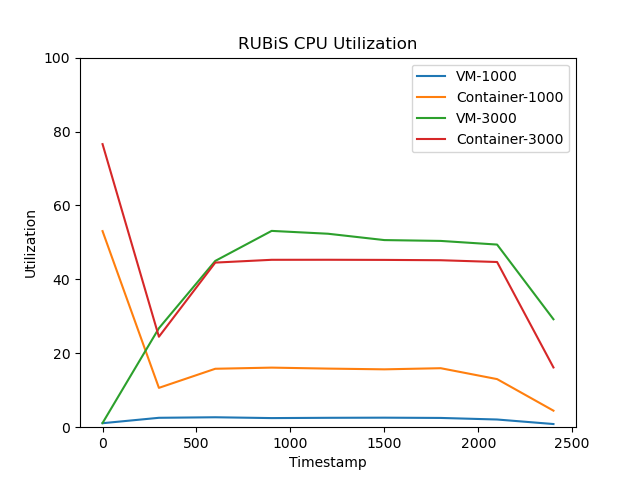
\includegraphics[width=1.1\linewidth]{rubis_cpu_util.png}
  \caption{RUBiS CPU utilization}
  \label{fig:rub1}
\end{subfigure}%
\begin{subfigure}{.5\textwidth}
  \centering
  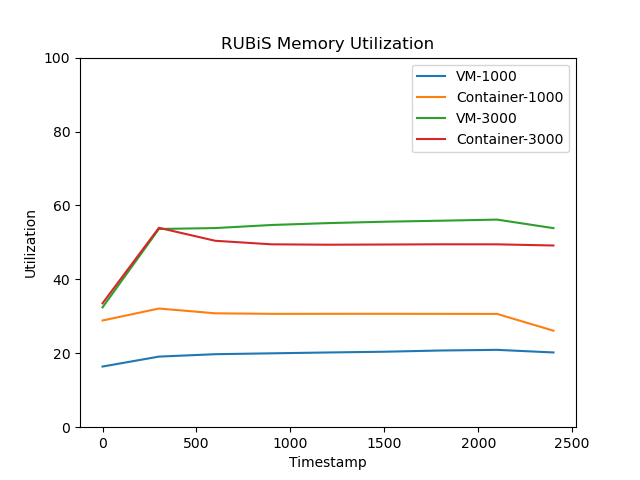
\includegraphics[width=1.1\linewidth]{rubis_mem_util.png}
  \caption{RUBiS Memory utilization}
  \label{fig:rub2}
\end{subfigure}
\caption{RUBiS}
\label{fig:rubis}
\end{figure}

Though memory and CPU usage does increase with the increase of number of concurrent clients, the increment is not linear in every aspect. The VM’s CPU usage increases by a factor of about 20, but the containers have about a 3x increment, and in the case of memory, VM's seems to have a linear relationship but not the containers. Though the VM's seem to utilize less memory and CPU for 1000 clients, it is not the case at the level of 3000 concurrent clients as containers have a lesser memory and CPU consumption at that level. As we have kept all the CPU and memory equal for both VM's and containers, the only thing we think of this inconsistency is related to disk as explained by micro-benchmarks.

Other than the CPU and memory utilization Table 1 represents a brief summary related to the number of requests made by each instance with 1000 and 3000 clients respectively. One thing to notice here is with the increase in number of clients, VM's increase the number of requests exponentially when compared with ECS. We also tuned the number of clients parameter further and realized that containers could not handle more than 3000 clients with the current configuration, while VM's could go up to a level of 5000 clients keeping the configurations unchanged.

\begin{center}
\captionsetup[table]{position=bottom}
 \begin{tabular}{||c c c ||} 
 \hline
 Instance \& Clients & Total number of requests & Average throughput  \\ [0.5ex] 
 \hline
 ECS - 1000 & 389165 & 161 req/s  \\ 
 \hline
 EC2 - 1000 & 34971 & 14 req/s \\ 
 \hline
 ECS - 3000 & 1192166 & 496 req/s  \\ 
 \hline
 EC2 - 3000 & 1062825 & 452 req/s \\ 
  \hline

\end{tabular}
\captionof{table}{ECS \& EC2 Summary} 

\end{center}

\subsection{GBM-perf}

The first step to benchmarking with GBM-perf was to setup the images. For Docker this was straightforward, since the source code included a Dockerfile to build from. The VM image was more involved, requiring backtracing the commands from the base images (rocker/tidyverse was the base image). After several test runs, it was discovered that at least 16 GB of memory is required to run all the GBM-perf benchmarks. An m5.xlarge instance was used for EC2, along with a gp2 (SSD) EBS volume. For Fargate, memory was set to 16 GB, along with 4 vCPUs. Fargate gets 20 GB of unspecified ephemeral storage, though from the benchmarks it appears to be an SSD. More storage can be added with AWS EFS.

\begin{figure}[hbt!]
\centering
\begin{subfigure}{.5\textwidth}
  \centering
  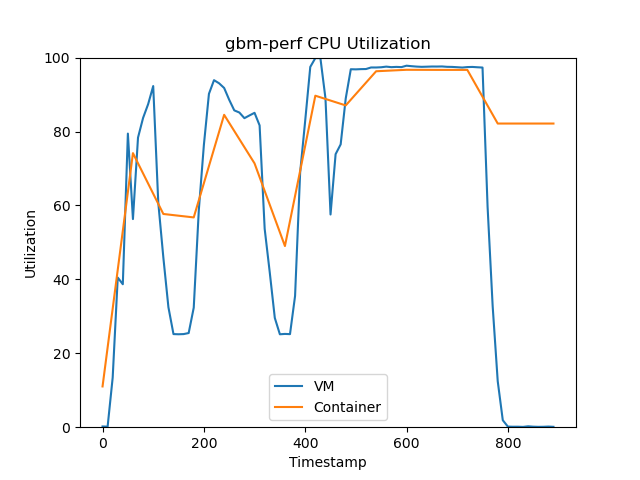
\includegraphics[width=1.1\linewidth]{gbmperf_cpu_util.png}
  \caption{CPU}
  \label{fig:gbmperfu1}
\end{subfigure}%
\begin{subfigure}{.5\textwidth}
  \centering
  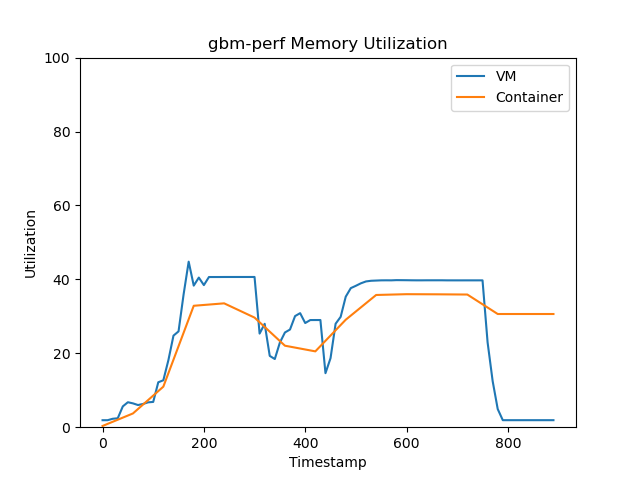
\includegraphics[width=1.1\linewidth]{gbmperf_mem_util.png}
  \caption{Memory}
  \label{fig:gbmperfu2}
\end{subfigure}
\caption{GBM-perf-Utilizations}
\label{fig:gbmperfutilizations}
\end{figure}

GBM-perf was run 5 times on each platform, each producing CPU and memory metrics. The average was taken among these and graphed in a line plot (figure 2). In terms of CPU utilization, the results were very similar for both, with the VM being slightly higher. This is likely due to the VM having better sequential read speed, combined with a more powerful processor, allowing it to process more data at once, resulting in higher utilization. The VM uses a Xeon Platinum 8175M with a clockspeed of 3.1 GHz, while the container uses a Xeon E5-2686 at 2.3 GHz. The memory utilization shows a similar pattern, with the VM being slightly higher. This is likely caused by idle consumption from background processes.

\begin{figure}[hbt!]
  \centering
  \begin{subfigure}{.5\textwidth}
    \centering
    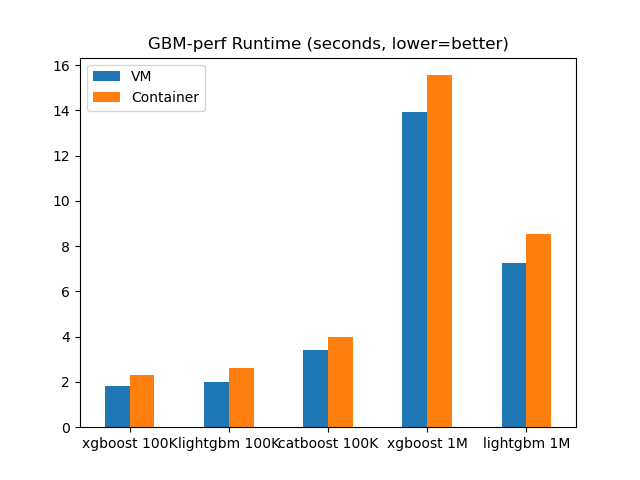
\includegraphics[width=1.1\linewidth]{gbmperf_runtime_1.png}
    \caption{runtime-1}
    \label{fig:gbmperfr1}
  \end{subfigure}%
  \begin{subfigure}{.5\textwidth}
    \centering
    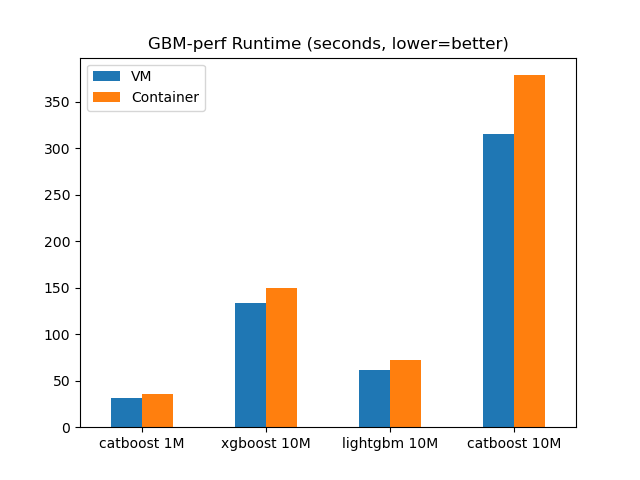
\includegraphics[width=1.1\linewidth]{gbmperf_runtime_2.png}
    \caption{runtime-2}
    \label{fig:gbmperfr2}
  \end{subfigure}
  \caption{GBM-perf-runtime}
  \label{fig:rubis}
\end{figure}

The primary result of the GBM-perf benchmark was the runtime. The benchmark also produced the training accuracy, but was deterministic, since both use the same dataset. In all cases the VM outperformed the container, with the average runtime being 15.19\% faster. For example, for the catboost library on the 10M dataset, the VM took 316 seconds, while the container took 379 seconds. This discrepancy is most likely attributed to the speed and ISA of the CPU, as well as the sequential read speed of the disk. Not considering other factors, this benchmark concludes that EC2 is the preferable service for CPU dominant workloads.


\subsection{Sysbench}

As we already explained, we selected Sysbench to carry out the micro-benchmarking of VM's and containers. In addition to comparing the different measurements between the two systems, it helped us to explain the results that we obtained from the macro-benchmarking.

First we tested for the CPU using the brute-force prime number search. Figure 4(a) represents the CPU utilization during the test. During the first half of the test, both the containers and VM's utilized almost 100\% of the CPU, but this fluctuates in next phase. Figure 4(b) represents the time that it took to finish the test, with VM's clearly completing the test quicker than the containers. Among the two VM's used, the c5 instance, which is designed for compute intensive workloads, performed better than the m5 instance which is typically used for general purpose workloads. 

\begin{figure}[hbt!]
\centering
\begin{subfigure}{.5\textwidth}
  \centering
  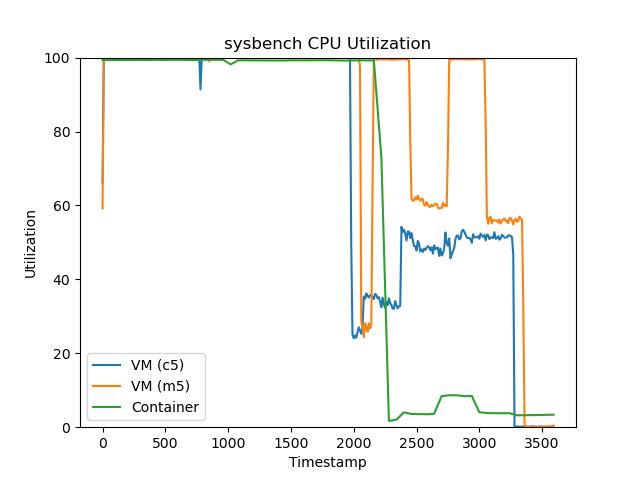
\includegraphics[width=1.1\linewidth]{sysbench_cpu.png}
  \caption{Sysbench CPU utilization}
  \label{fig:sysb1}
\end{subfigure}%
\begin{subfigure}{.5\textwidth}
  \centering
  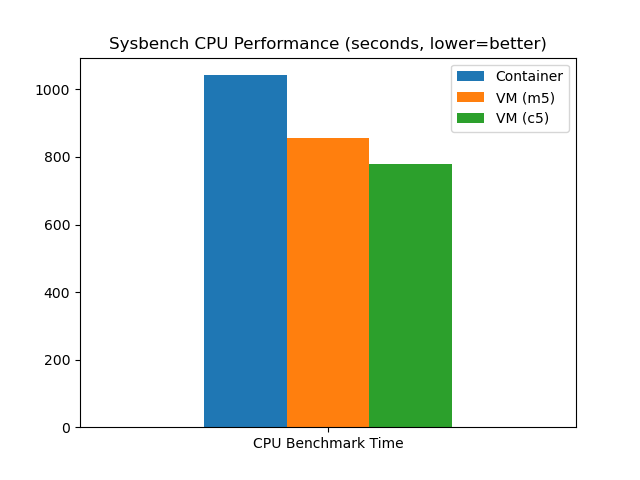
\includegraphics[width=1.1\linewidth]{sysbench_cpu_bar.png}
  \caption{Sysbench CPU performance}
  \label{fig:sysb2}
\end{subfigure}
\caption{Sysbench - CPU}
\label{fig:rubis}
\end{figure}

When using the memory test in Sysbench, it will allocate a memory buffer and then read or write from it. According to the Figure 5, the results were as expected, with the memory reads being much faster than the memory writes. When comparing with the VM's and containers, VM's seem to perform much better than the containers for reads but they seem to have identical performance for the writes. The memory utilization values are unnoticeable, as the block size used in the test was just 2MB which is negligible when compared to the available memory. 

\begin{figure}[H]
\centering
\begin{subfigure}{.5\textwidth}
  \centering
  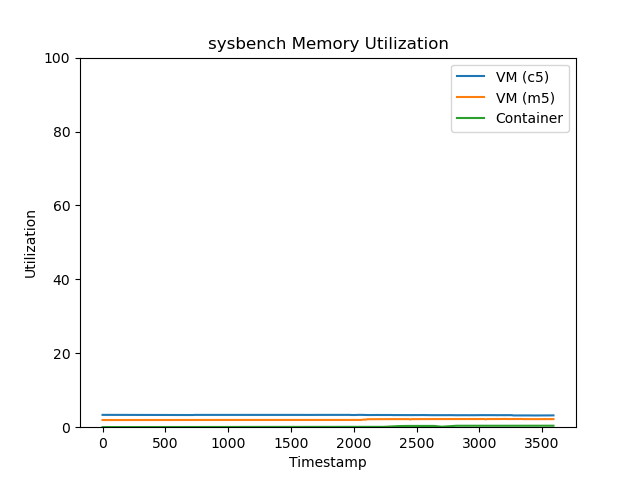
\includegraphics[width=1.1\linewidth]{sysbench_mem.png}
  \caption{Sysbench memory utilization}
  \label{fig:sysbm1}
\end{subfigure}%
\begin{subfigure}{.5\textwidth}
  \centering
  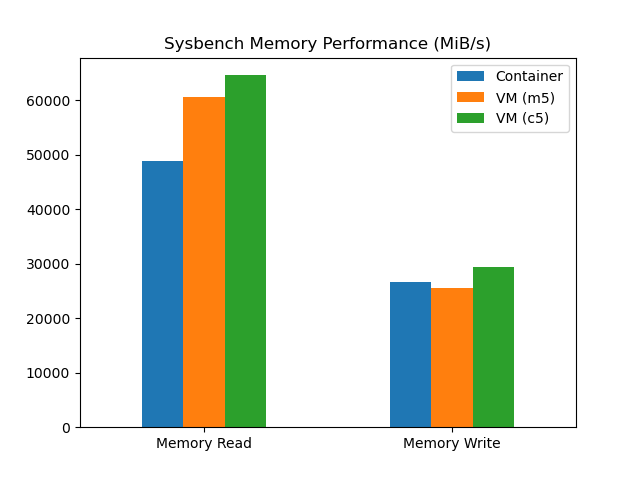
\includegraphics[width=1.1\linewidth]{sysbench_mem_bar.png}
  \caption{Sysbench memory performance}
  \label{fig:sysbm2}
\end{subfigure}
\caption{Sysbench - Memory}
\label{fig:rubis}
\end{figure}

\begin{figure}[H]
\centering
  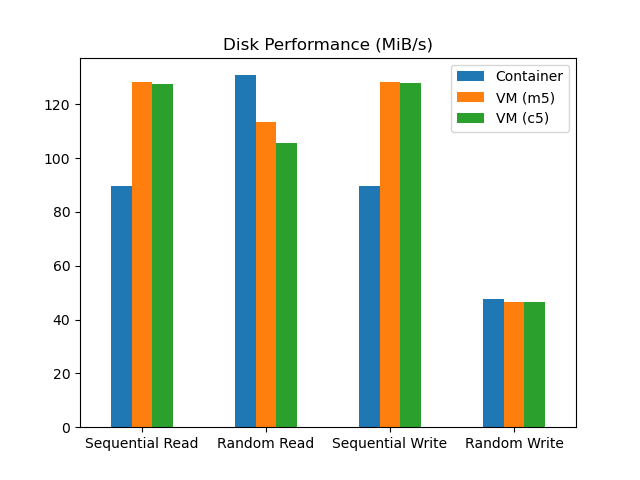
\includegraphics[width=0.55\linewidth]{sysbench_disk.png}
  \caption{Sysbench - Disk}
  \label{fig:disk}
\end{figure}

Finally, comparison between the disk performance of the two systems are shown in Figure 6. In the case of sequential reads, data is stored in consecutive blocks where in the case of random read, data is stored in random blocks all over the drive.  Accessing data sequentially is much faster than accessing it randomly because of the way in which the disk hardware works. In the case of VM's Figure 6 clearly support this idea where both the sequential reads and writes performs much faster than that of random reads and writes for both VM types used. However, in the case of containers, random read has much higher performances than the sequential reads. We believe the reason for this was either Fargate's SSD model or the docker storage driver.


\subsection{Other measures}

In addition to the benchmarks, we considered some other information for our comparison. First we averaged the two metrics at idle time. Figure 7 confirmed that our speculation about the memory and CPU of VM's would have non zero values while the containers would have almost zero values for both the cases.   

\begin{figure}[H]
\centering
\begin{subfigure}{.5\textwidth}
  \centering
  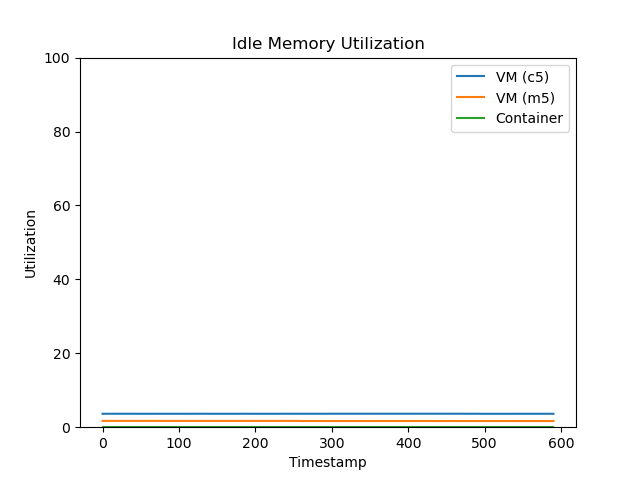
\includegraphics[width=1.1\linewidth]{idle_mem.png}
  \caption{Memory idle}
  \label{fig:idlemem}
\end{subfigure}%
\begin{subfigure}{.5\textwidth}
  \centering
  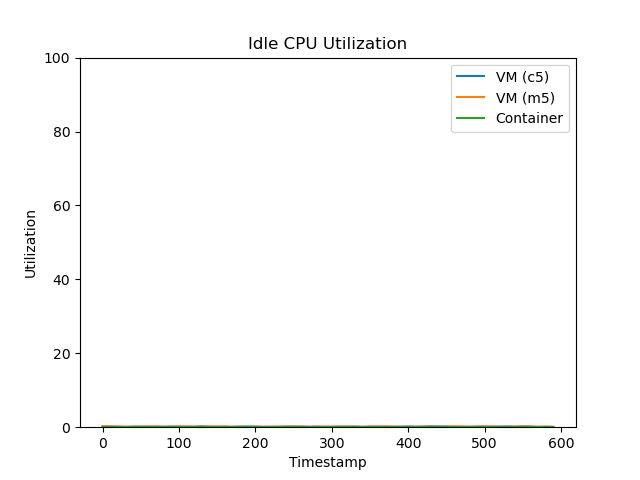
\includegraphics[width=1.1\linewidth]{idle_cpu.png}
  \caption{CPU idle}
  \label{fig:idlecpu}
\end{subfigure}
\caption{Idle measures}
\label{fig:rubis}
\end{figure}

\begin{table}[hbt!]
    \begin{tabular}{|l|l|l|l|l|l|l|}
    \hline
                           & m5.xlarge & ECS     & c5.xlarge  & ECS     & t2.small  & ECS     \\ \hline
    Resources (vCPU / RAM) & 4/16      & 4/16    & 4/8        & 4/8     & 1/2       & 1/2     \\ \hline
    Cost / hr              & 0.192     & 0.23304 & 0.17       & 0.19748 & 0.023     & 0.04937 \\ \hline
    \end{tabular}
    \captionof{table}{cost comparisons} 
\end{table}

Measuring the startup time for EC2 instances involved writing a startup script that would print the timestamp right after the instance startup request was sent to AWS. The VM was then setup to print a timestamp when a custom systemd service was started on boot. This difference represents the effective time it would to successfully scale a service. Containers were measured similarly by taking the difference between the time the ECS service was updated with a higher number of replicas to when the entry command was run. We tested going from 0 to 1 replicas and from 1 to 3 replicas, but the startup time was the same. Despite assuming the opposite, VMs turned out to startup faster in all cases. This is due to how Fargate operates, as described earlier. Several different scenarios were tested. For EC2 we measure the t2.small instance type with an 8 GB EBS volume for both a plain Ubuntu image and RUBiS. We also tested GBM-perf on a m5.xlarge. These configurations would account for instance size, startup processes, and disk size.

\begin{figure}[H]
  \centering
    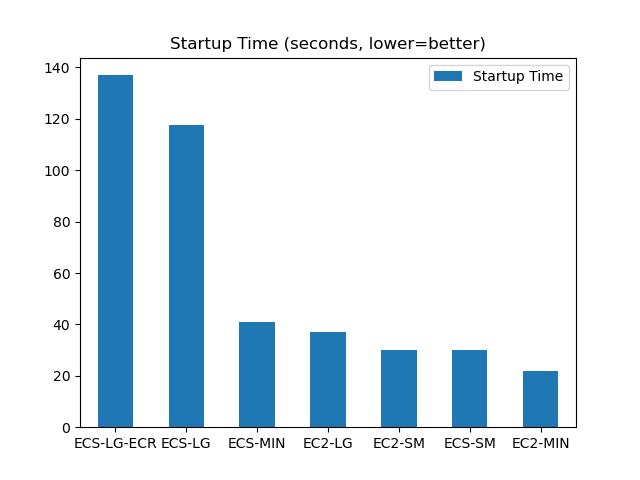
\includegraphics[width=0.55\linewidth]{startup_time.png}
    \caption{Startup Time}
    \label{fig:disk}
\end{figure}

The measured times were 22, 30, and 37 seconds (shown in figure 8). We found a smaller disk size resulted in a faster startup time due to having less data that needs to be copied. Additionally, the startup tasks of the RUBiS image took time to complete. For Fargate, we had the following configurations ([image, size, vCPU/memory]): [alpine, 3 MB, 4/16], [alpine, 3 MB, 1/2], [gbm-perf, 1.5 GB on ECR, 4/16], [gbm-perf, 1.5 GB, 4/16]. The resulting times for these were 30, 37, 117.5, and 137 seconds averaged across 3 runs. The longer time to start a container with lower resources was unexpected, and may be caused by the way Fargate does scheduling. We ran this another 3 times to verify, but got the same result. Larger images sizes have a drastic impact on startup time, since these need to be pulled from the Internet and are not cached locally. Images stored on ECR take even longer. From these findings, EC2 is preferred over Fargate for scaling unless working with small images. Another option would be to use ECS with the image caching feature, though this requires managing EC2 instances manually.

Lastly, the cost data in Table 2 shows that EC2 instances cost less per resource. m5.xlarge instances cost \$0.192 per hour, while the same number of vCPUs and GB of RAM costs \$0.233 per hour. For small instances the comparison is even more extreme with \$0.023 for a t2.small and \$0.049 for a similar Fargate container, over twice as much. This concludes EC2 instances are more cost-effective for static workloads, and when considering the scalability of both services, for dynamic workloads as well.

\vspace{3mm} %3mm vertical space


\section{Conclusion}

In conclusion of our study, we could not explicitly say that one virtualization technology is superior to other, as it depends on the different environments in which they operate, and the ultimate decision will depend on the user's specific needs. 

Virtual machines are very suitable for tasks that require high capacity throughput and disk locality, such as relational databases. If there is not much traffic and if the requirement for scaling is lower, then VM's would be a better option, as it's very easy to get started with and does not require resources that would typically be needed in a container environment. Other than that, if you need to build a legacy system which manages multiple applications on a single server, and requires most resources and functionalities of an OS, then it would be better to go with VM's. Though it was claimed that VM's ensure a higher level of isolation and security than containers, with the use of technologies like Firecracker, containers can have just as much isolation and security as VM's.

In the case of containers, they are most useful and easier to manage for stateless services. Containers are also a perfect fit for micro-service architectures where the application structure is a collection of services that are loosely coupled, highly maintainable, and easily testable. Presence of state of art orchestration systems like Kubernetes will also increase the manageability of these architectures. Finally, containers would also be suitable for technologies such as AWS Lambda, which executes your program logic on-demand, and have the capability to handle burst workloads, from a few requests to thousands per second without having to pay much.

\vspace{3mm} %3mm vertical space


\section{Division of Work}

\paragraph{Heshan}

\begin{itemize}
  \item Original RUBiS benchmark
  \item RUBiS modification for additional users
  \item Measurement of startup times for VMs
  \item Report: RUBiS key ideas and evaluation, Sysbench, Conclusion
\end{itemize}

\paragraph{Michael}

\begin{itemize}
  \item GBM-perf benchmark
  \item Sysbench, idle, and cost data
  \item Measurement of startup times for containers
  \item Report: GBM-perf key ideas and evaluation, related work, startup times and cost
\end{itemize}


\printbibliography

\end{document}
